\documentclass{article}
\usepackage{algorithm}
\usepackage{float} % Add this line in the preamble
\usepackage{algpseudocode}
\usepackage{graphicx}
\usepackage{amsmath, amssymb}

\title{Derandomized Color Coding via Two-Stage K-Perfect Hashing}
\author{Your Name}
\date{\today}

\begin{document}

\maketitle

\begin{abstract}
    This paper presents a derandomized color coding algorithm using two-stage $k$-perfect hash families for finding colorful paths in graphs. We describe the construction of polynomial hash functions, the composition of two-stage hash families, and the dynamic programming approach for detecting colorful paths.
\end{abstract}

\section{Introduction}
Color coding is a powerful technique for detecting small subgraphs, such as paths or cycles, in large graphs. The derandomized version uses $k$-perfect hash families to systematically assign colors, ensuring coverage of all possible colorings.


\section{ Single Stage Hashing using GF(p)}

\begin{algorithm}[H]
    \caption{Derandomized Color Coding to Detect Colorful Paths of Length $k$}
    \begin{algorithmic}[1]
        \State \textbf{Input:} Graph $G = (V, E)$, target path length $k$
        \State \textbf{Output:} \texttt{True} if a colorful path of length $k$ exists, else \texttt{False}
        \Function{DerandomizedColorCoding}{$G, k$}
        \State $n \gets |V|$
        \State Construct $k$-perfect hash family $\mathcal{H}$ using:
        \For{$a = 1$ to $k$}
        \For{$b = 0$ to $k-1$}
        \State Add $h_{a,b}(v) = ((a \cdot v + b) \mod p) \mod k + 1$ to $\mathcal{H}$ \Comment{$p > n$, prime}
        \EndFor
        \EndFor
        \For{each hash function $h \in \mathcal{H}$}
        \State Assign colors $c[v] \gets h(v)$ for all $v \in V$
        \State Initialize DP table $dp[v][S] \gets \texttt{false}$ for $v \in V, S \subseteq \{1, \dots, k\}$
        \For{$v \in V$}
        \State $dp[v][\{c[v]\}] \gets \texttt{true}$
        \EndFor
        \For{$\ell = 1$ to $k-1$}
        \For{$v \in V$}
        \For{each subset $S \subseteq \{1,\dots,k\}$ of size $\ell$}
        \If{$dp[v][S] = \texttt{true}$}
        \For{each $u \in \text{neighbors}(v)$}
        \If{$c[u] \notin S$}
        \State $dp[u][S \cup \{c[u]\}] \gets \texttt{true}$
        \EndIf
        \EndFor
        \EndIf
        \EndFor
        \EndFor
        \EndFor
        \For{$v \in V$}
        \If{$dp[v][\{1, \dots, k\}] = \texttt{true}$}
        \State \Return \texttt{true}
        \EndIf
        \EndFor
        \EndFor
        \State \Return \texttt{false}
        \EndFunction
    \end{algorithmic}
\end{algorithm}

\section{Polynomial Hash Function Construction}
\begin{algorithm}[H]
    \caption{Polynomial Hash Function Construction}
    \begin{algorithmic}[1]
        \Require Degree $k - 1$, prime $p$
        \Ensure A hash function $h(x)$ over $\text{GF}(p)$
        \State Generate $k$ random coefficients $a_0, a_1, \ldots, a_{k-1} \in \{0, \ldots, p - 1\}$
        \While{$k > 1$ and $a_{k-1} = 0$}
        \State Re-sample $a_{k-1}$ from $\{0, \ldots, p - 1\}$
        \EndWhile
        \State Define $h(x) = a_0 + a_1 x + a_2 x^2 + \ldots + a_{k-1}x^{k-1}$ \textbf{mod} $p$
        \State Use Horner's Rule to evaluate $h(x)$ efficiently
    \end{algorithmic}
\end{algorithm}

\section{K-Perfect Hash Family Construction}
\begin{algorithm}[H]
    \caption{K-Perfect Hash Family Construction}
    \begin{algorithmic}[1]
        \Require $k$: range size, $n$: universe size, $m$: number of hash functions
        \Ensure Family of $m$ polynomial hash functions
        \State Find smallest prime $p > \max(n, k)$
        \For{$i = 1$ to $m$}
        \State Generate a polynomial hash of degree $k - 1$ over $\text{GF}(p)$
        \EndFor
        \State Store all $m$ functions as the hash family
    \end{algorithmic}
\end{algorithm}

\section{Two-Stage K-Perfect Hash Composition}
\begin{algorithm}[H]
    \caption{Two-Stage K-Perfect Hash Composition}
    \begin{algorithmic}[1]
        \Require Stage-1: maps $[1,n] \rightarrow [0,k^2{-}1]$, Stage-2: maps $[0,k^2{-}1] \rightarrow [0,k{-}1]$
        \Ensure Composed hash maps $v \in [1,n]$ to color $\in [0,k{-}1]$
        \State Construct stage-1 hash family with $2k\lceil \log_2 n \rceil$ functions
        \State Construct stage-2 hash family with $k^2$ functions
        \Function{TwoStageHash}{$v, i, j$}
        \State $intermediate \gets$ Stage1Hash[$i$]$(v) \mod k^2$
        \State \Return Stage2Hash[$j$]$(intermediate) \mod k$
        \EndFunction
    \end{algorithmic}
\end{algorithm}


\begin{algorithm}[H]
    \caption{Two-Stage Polynomial Hash Function for Coloring}
    \begin{algorithmic}[1]
        \Require Vertex identifier $v \in \{1, \ldots, n\}$, indices $i_1$, $i_2$, integer $k$
        \Ensure Composed hash maps $v \in [1, n]$ to color $\in [0, k-1]$
        \Statex
        \State \textbf{// Stage 1: Construct family of $m_1 = 2k\lceil \log_2 n \rceil$ polynomial hash functions $f^{(1)}_{i_1}$}
        \State Find smallest prime $p_1 > \max(n, k)$
        \For{each $f^{(1)}_{i_1}$}
            \State Generate $k$ random coefficients $a_0, a_1, \ldots, a_{k-1} \in \{0, \ldots, p_1 - 1\}$
            \While{$k > 1$ and $a_{k-1} = 0$}
                \State Re-sample $a_{k-1}$ from $\{0, \ldots, p_1 - 1\}$
            \EndWhile
            \State Define $f^{(1)}_{i_1}(x) = a_0 + a_1 x + \ldots + a_{k-1}x^{k-1} \bmod p_1$
        \EndFor
        \Statex
        \State \textbf{// Stage 2: Construct family of $m_2 = k^2$ polynomial hash functions $f^{(2)}_{i_2}$}
        \State Find smallest prime $p_2 > k^2$
        \For{each $f^{(2)}_{i_2}$}
            \State Generate $k$ random coefficients $b_0, b_1, \ldots, b_{k-1} \in \{0, \ldots, p_2 - 1\}$
            \While{$k > 1$ and $b_{k-1} = 0$}
                \State Re-sample $b_{k-1}$ from $\{0, \ldots, p_2 - 1\}$
            \EndWhile
            \State Define $f^{(2)}_{i_2}(y) = b_0 + b_1 y + \ldots + b_{k-1}y^{k-1} \bmod p_2$
        \EndFor
        \Statex
        \Function{Color}{$v, i_1, i_2$}
            \State $t \gets f^{(1)}_{i_1}(v) \bmod k^2$
            \State \Return $f^{(2)}_{i_2}(t) \bmod k$
        \EndFunction
    \end{algorithmic}
    \end{algorithm}
    



\begin{algorithm}
    \caption{Two-Stage LFSR-Based Color Hashing for $k$-Perfect Hashing}
    \begin{algorithmic}[1]
        \Require Vertex identifier \( v \in \{1, \dots, n\} \), indices \( i_1 \), \( i_2 \)
        \Ensure Color \( c(v) \in \{1, \dots, k\} \)

        \State Define tap mask \( T = \texttt{0x80200003} \) for primitive polynomial
        \State Define bit widths \( m = 32 \), \( l_1 = \lceil \log_2 (k^2) \rceil \), \( l_2 = \lceil \log_2 k \rceil \)
        \State Initialize two LFSR hash families:
        \Statex \quad \( H_1 \gets \text{LFSRHashFamily}(T, m, 2k \cdot \lceil \log_2 n \rceil) \)
        \Statex \quad \( H_2 \gets \text{LFSRHashFamily}(T, m, k^2) \)

        \Function{Color}{$v, i_1, i_2$}
        \State \( h_1 \gets \text{Hash}(H_1, i_1, v, l_1) \bmod k^2 \)
        \State \( h_2 \gets \text{Hash}(H_2, i_2, h_1, l_2) \bmod k \)
        \State \Return \( h_2 + 1 \)
        \EndFunction

        \Function{Hash}{family, func\_idx, steps, $\ell$}
        \State \( s \gets \text{Seed}[func\_idx \bmod \text{family.size}] \)
        \For{\( j = 1 \) to \texttt{steps}}
        \State \( s \gets \textsc{LFSRNext}(s, T) \)
        \EndFor
        \State \( h \gets 0 \)
        \For{\( i = 0 \) to \( \ell - 1 \)}
        \State \( h \gets (h \ll 1) \lor (s \& 1) \)
        \State \( s \gets \textsc{LFSRNext}(s, T) \)
        \EndFor
        \State \Return \( h \)
        \EndFunction

        \Function{LFSRNext}{state, taps}
        \State \( \texttt{lsb} \gets \texttt{state} \& 1 \)
        \State \( \texttt{state} \gets \texttt{state} \gg 1 \)
        \If{\( \texttt{lsb} = 1 \)}
        \State \( \texttt{state} \gets \texttt{state} \oplus \texttt{taps} \)
        \EndIf
        \State \Return \( \texttt{state} \)
        \EndFunction

    \end{algorithmic}
\end{algorithm}

% \begin{algorithm}
%     \caption{Two-Stage LSFR Hash Construction for $k$-Perfect Hashing}
%     \begin{algorithmic}[1]
%         \Require Vertex identifier \( v \), Stage 1 index \( i \), Stage 2 index \( j \)
%         \Ensure Deterministic color \( c(v) \in \{0, \ldots, k-1\} \)

%         \State Define LSFR parameters: bit width \( r = \log_2 n \), output size \( k \)
%         \State Define fixed tap masks: \( \text{TapMasks} = [t_1, t_2, \ldots, t_m] \)

%         \Function{TwoStageHash}{$v, i, j$}
%         \State \( \text{seed}_1 \gets \text{RandomSeed}(i) \)
%         \State \( \text{tap}_1 \gets \text{TapMasks}[i \bmod m] \)
%         \State \( h_1 \gets \text{LSFR}(v, \text{seed}_1, \text{tap}_1, r) \mod m \) \Comment{Stage 1 hash to intermediate space}

%         \State \( \text{seed}_2 \gets \text{RandomSeed}(j) \)
%         \State \( \text{tap}_2 \gets \text{TapMasks}[j \bmod m] \)
%         \State \( h_2 \gets \text{LSFR}(h_1, \text{seed}_2, \text{tap}_2, r) \mod k \) \Comment{Stage 2 hash to final color space}

%         \State \Return \( h_2 \)
%         \EndFunction

%         \Function{LSFR}{input, seed, tap, bitWidth}
%         \State Initialize \texttt{state} \( \gets \text{seed} \)
%         \For{\( \ell = 1 \) to \texttt{input} }
%         \State \texttt{feedback} \( \gets 0 \)
%         \For{\( i = 0 \) to \texttt{bitWidth} - 1}
%         \If{(\( \texttt{tap} \gg i \) \textbf{AND} 1) = 1}
%         \State \texttt{feedback} \( \gets \texttt{feedback} \oplus ((\texttt{state} \gg i) \textbf{AND} 1) \)
%         \EndIf
%         \EndFor
%         \State \texttt{state} \( \gets ((\texttt{state} \ll 1) \textbf{OR} \texttt{feedback}) \textbf{AND} ((1 \ll \texttt{bitWidth}) - 1) \)
%         \EndFor
%         \State \Return \texttt{state}
%         \EndFunction

%         \Function{RandomSeed}{index}
%         \State Use fixed PRNG to deterministically generate a seed based on \texttt{index}
%         \State \Return a 16-bit integer in \([1, 2^{16} - 1]\)
%         \EndFunction

%     \end{algorithmic}
% \end{algorithm}

% \section{LSFR Algorithm}
% \begin{algorithm}[H]
%     \caption{Two-Stage LSFR Hashing and Derandomized Color Coding}
%     \begin{algorithmic}[1]
%         \Require Graph $G = (V, E)$, path length $k$
%         % \Ensure Whether $G$ contains a simple path of length $k$
%         \Ensure Composed hash maps $v \in [1,n]$ to color $\in [0,k{-}1]$

%         \Statex
%         \Function{LSFR}{$x$, seed, taps, bitWidth}
%         \State $state \gets seed$
%         \For{$i = 0$ to $x-1$}
%         \State $feedback \gets 0$
%         \For{$j = 0$ to $bitWidth - 1$}
%         \If{$(taps \gg j) \& 1 = 1$}
%         \State $feedback \gets feedback \oplus ((state \gg j) \& 1)$
%         \EndIf
%         \EndFor
%         \State $state \gets ((state \ll 1) | feedback) ~\&~ ((1 \ll bitWidth) - 1)$
%         \EndFor
%         \State \Return $state$
%         \EndFunction

%         \Statex
%         \Function{TwoStageHash}{$v, i, j$}
%         \State $h_1 \gets \text{LSFR}(v, \text{seed}_i, \text{tap}_i, 16) \bmod (k \cdot k)$
%         \State $h_2 \gets \text{LSFR}(h_1, \text{seed}_j, \text{tap}_j, 16) \bmod k$
%         \State \Return $h_2$ \Comment{Color in $\{0, \dots, k-1\}$}
%         \EndFunction

%     \end{algorithmic}
% \end{algorithm}

\section{Derandomized Color Coding Algorithm}
\begin{algorithm}[H]
    \caption{Derandomized Color Coding with Two-Stage Hashing}
    \begin{algorithmic}[1]
        \Require Graph $G = (V, E)$ with vertices $V = \{1, \dots, n\}$, target path length $k$
        \Ensure Return true if a colorful path of length $k$ exists
        \State Build $\text{TwoStageKPerfectHash}(k, n)$
        \For{each $i$ in stage-1 hashes}
        \For{each $j$ in stage-2 hashes}
        \State Assign colors $c(v) \gets \text{TwoStageHash}(v, i, j) + 1$ for all $v \in V$
        \If{\Call{HasColorfulPath}{$c$}}
        \State \Return true
        \EndIf
        \EndFor
        \EndFor
        \State \Return false
        \Function{HasColorfulPath}{$c$}
        \State Initialize $DP[v][S] \gets$ false for all $v \in V$, $S \subseteq \{1,\ldots,k\}$
        \For{each $v \in V$}
        \State $DP[v][\{c(v)\}] \gets$ true
        \EndFor
        \For{$len = 1$ to $k - 1$}
        \For{each $v \in V$}
        \For{each $S$ s.t. $|S| = len$ and $DP[v][S] = \text{true}$}
        \For{each neighbor $u$ of $v$ with $c(u) \notin S$}
        \State $DP[u][S \cup \{c(u)\}] \gets$ true
        \EndFor
        \EndFor
        \EndFor
        \EndFor
        \For{each $v \in V$}
        \If{$DP[v][\{1,2,\ldots,k\}] = \text{true}$}
        \State \Return true
        \EndIf
        \EndFor
        \State \Return false
        \EndFunction
    \end{algorithmic}
\end{algorithm}


% \section{Analysis}
% \begin{algorithm}
%     \caption{Two-Stage LSFR Hash Construction for $k$-Perfect Hashing}
%     \begin{algorithmic}[1]
%         \Require Vertex identifier \( v \), Stage 1 index \( i \), Stage 2 index \( j \)
%         \Ensure Deterministic color \( c(v) \in \{0, \ldots, k-1\} \)

%         \State Define LSFR parameters: bit width \( r = \log_2 n \), output size \( k \)
%         \State Define fixed tap masks: \( \text{TapMasks} = [t_1, t_2, \ldots, t_m] \)

%         \Function{TwoStageHash}{$v, i, j$}
%         \State \( \text{seed}_1 \gets \text{RandomSeed}(i) \)
%         \State \( \text{tap}_1 \gets \text{TapMasks}[i \bmod m] \)
%         \State \( h_1 \gets \text{LSFR}(v, \text{seed}_1, \text{tap}_1, r) \mod m \) \Comment{Stage 1 hash to intermediate space}

%         \State \( \text{seed}_2 \gets \text{RandomSeed}(j) \)
%         \State \( \text{tap}_2 \gets \text{TapMasks}[j \bmod m] \)
%         \State \( h_2 \gets \text{LSFR}(h_1, \text{seed}_2, \text{tap}_2, r) \mod k \) \Comment{Stage 2 hash to final color space}

%         \State \Return \( h_2 \)
%         \EndFunction

%         \Function{LSFR}{input, seed, tap, bitWidth}
%         \State Initialize \texttt{state} \( \gets \text{seed} \)
%         \For{\( \ell = 1 \) to \texttt{input} }
%         \State \texttt{feedback} \( \gets 0 \)
%         \For{\( i = 0 \) to \texttt{bitWidth} - 1}
%         \If{(\( \texttt{tap} \gg i \) \textbf{AND} 1) = 1}
%         \State \texttt{feedback} \( \gets \texttt{feedback} \oplus ((\texttt{state} \gg i) \textbf{AND} 1) \)
%         \EndIf
%         \EndFor
%         \State \texttt{state} \( \gets ((\texttt{state} \ll 1) \textbf{OR} \texttt{feedback}) \textbf{AND} ((1 \ll \texttt{bitWidth}) - 1) \)
%         \EndFor
%         \State \Return \texttt{state}
%         \EndFunction

%         \Function{RandomSeed}{index}
%         \State Use fixed PRNG to deterministically generate a seed based on \texttt{index}
%         \State \Return a 16-bit integer in \([1, 2^{16} - 1]\)
%         \EndFunction

%     \end{algorithmic}
% \end{algorithm}


\section{Analysis}
Results for different hash functions and their performance on different graph types are presented. 

For $K$= 8, the algorithm runs in $O(n^2)$ time. The two-stage hash family construction is efficient, and the dynamic programming approach ensures that we can find colorful paths in linear time.

\begin{figure}[H]
    \centering
    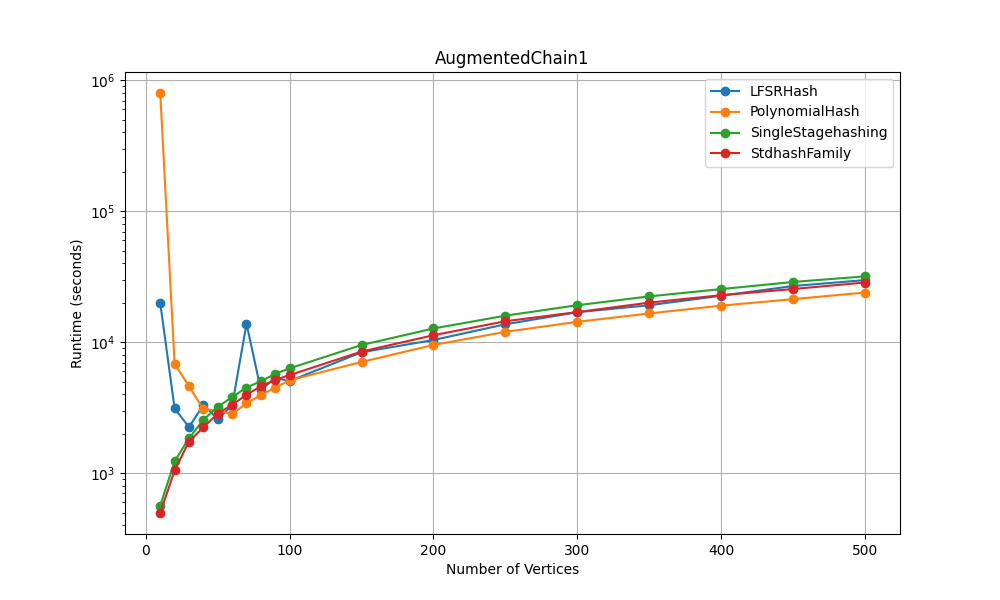
\includegraphics[width=0.8\linewidth]{figures/AugmentedChain1(fixedK).png}
    \caption{Augmented Chain Graph}
    \label{fig:AugmentedChain1}
\end{figure}

\begin{figure}[H]
    \centering
    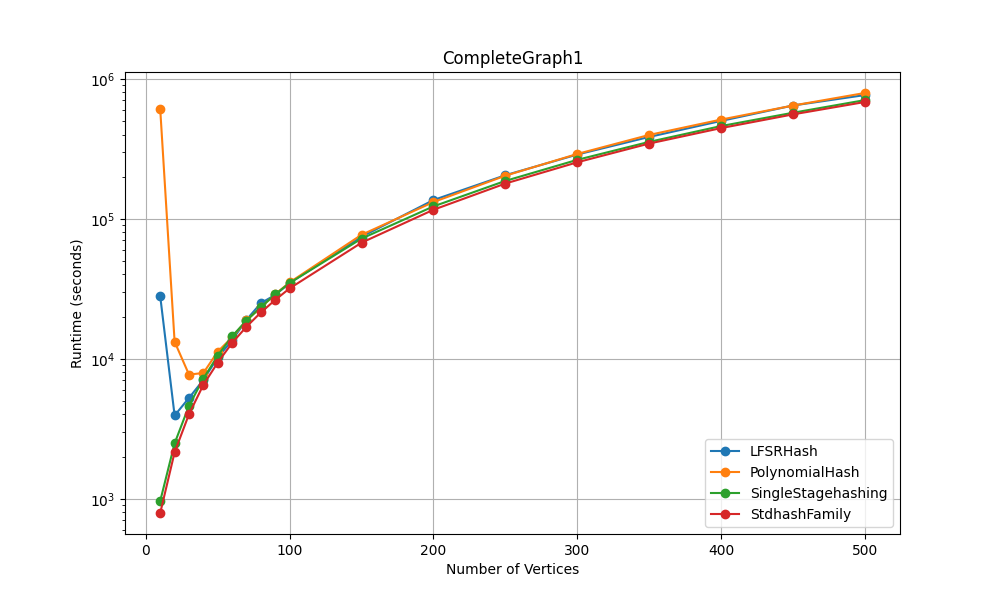
\includegraphics[width=0.8\linewidth]{figures/CompleteGraph1(fixedK).png}
    \caption{Complete Graph}
    \label{fig:CompleteGraph1}
\end{figure}

\begin{figure}[H]
    \centering
    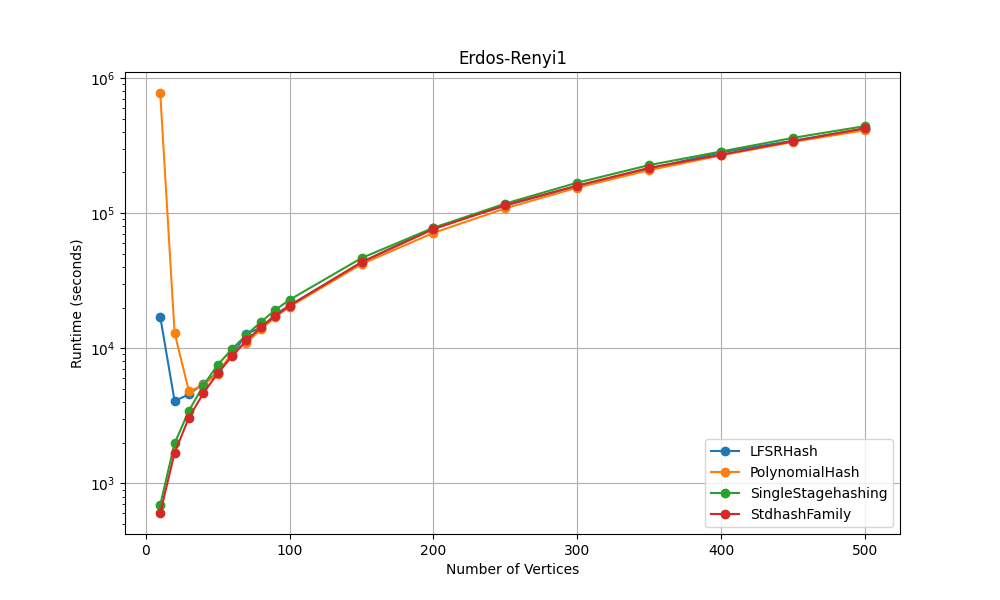
\includegraphics[width=0.8\linewidth]{figures/Erdos-Renyi1(fixedK).png}
    \caption{Erdos-Renyi Graph}
    \label{fig:ErdosRenyi1}
\end{figure}

\begin{figure}[H]
    \centering
    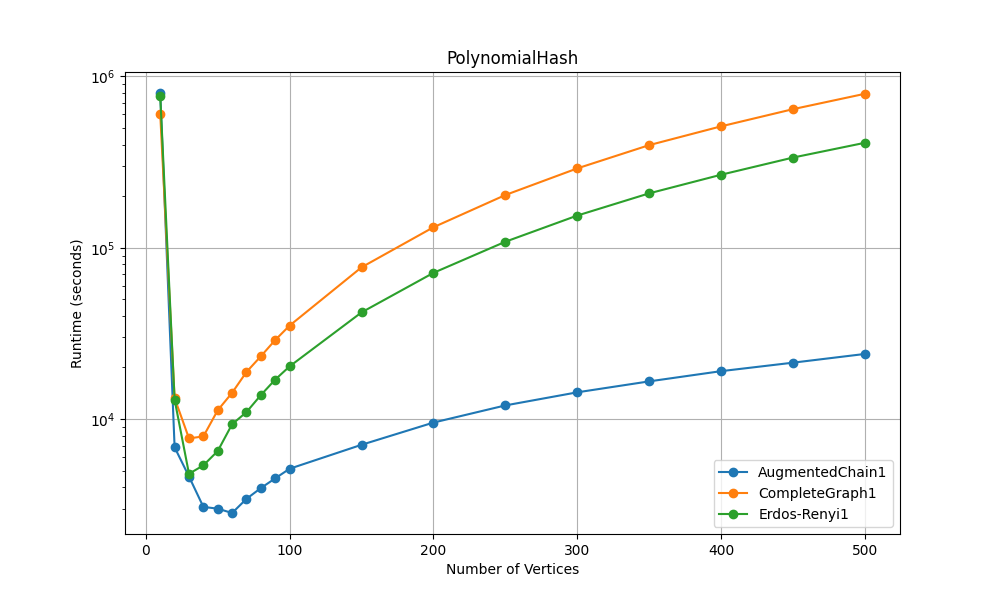
\includegraphics[width=0.8\linewidth]{figures/PolynomialHash(fixedK).png}
    \caption{Polynomial Hash Function}
    \label{fig:PolynomialHash}
\end{figure}

\begin{figure}[H]
    \centering
    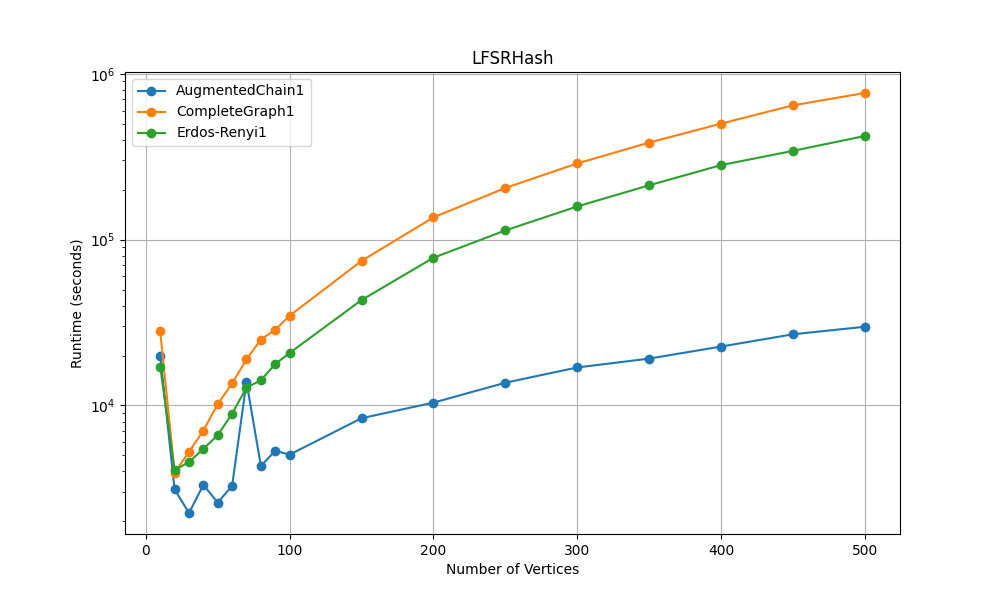
\includegraphics[width=0.8\linewidth]{figures/LFSRHash(fixedK).png}
    \caption{LFSR Hash Function}
    \label{fig:LFSRHash}
\end{figure}

\begin{figure}[H]
    \centering
    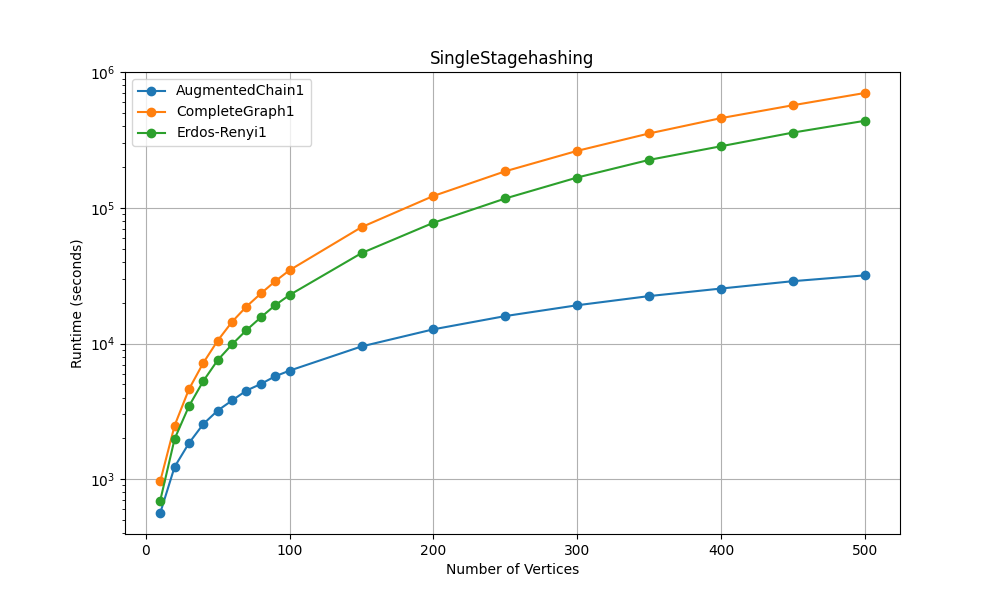
\includegraphics[width=0.8\linewidth]{figures/SingleStagehashing(fixedK).png}
    \caption{Single Stage Hashing}
    \label{fig:SingleStagehashing}
\end{figure}

\begin{figure}[H]
    \centering
    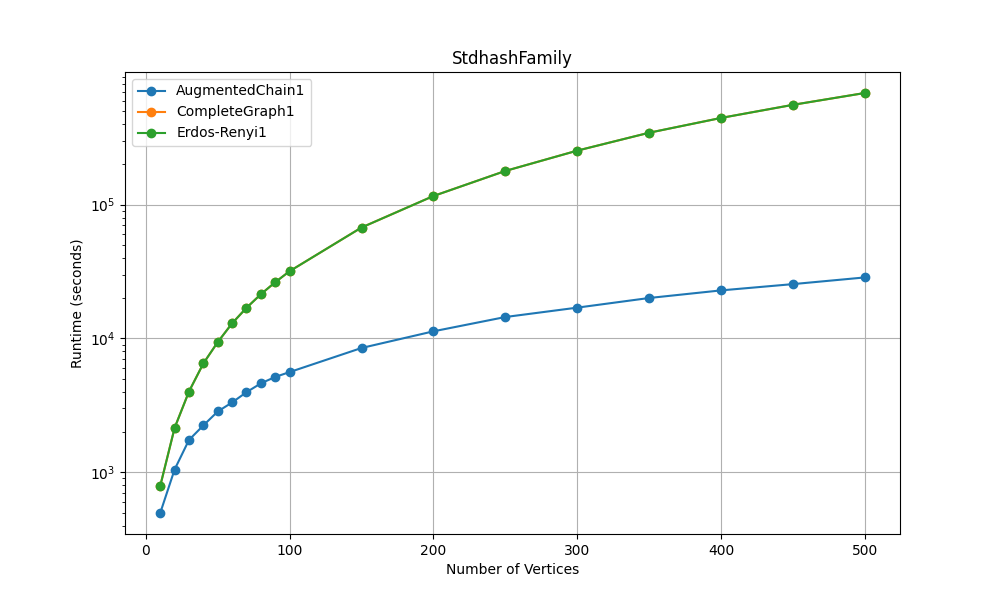
\includegraphics[width=0.8\linewidth]{figures/StdhashFamily(fixedK).png}
    \caption{Standard Hash Family}
    \label{fig:StdhashFamily}
\end{figure}

\begin{figure}[H]
    \centering
    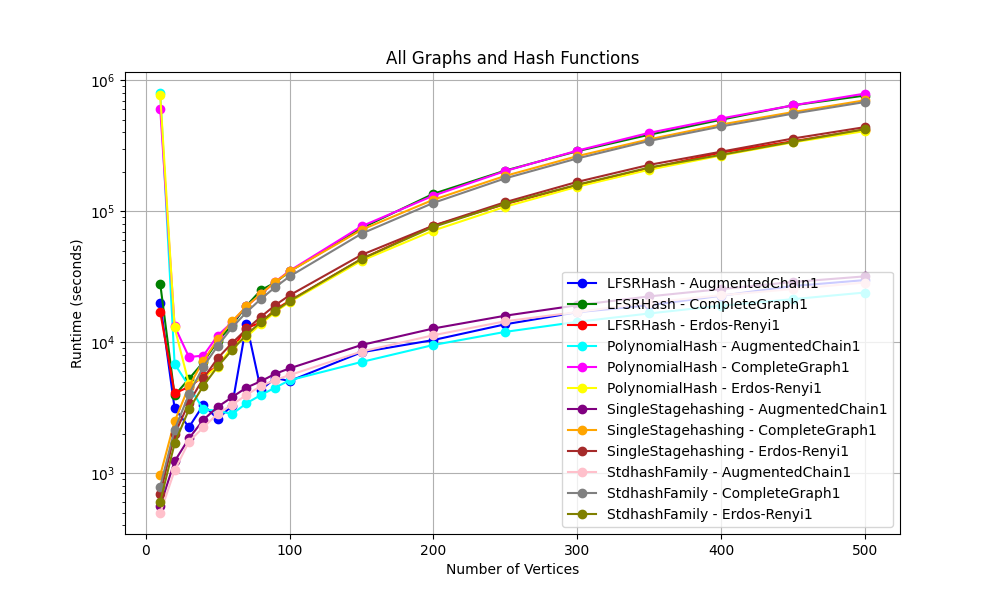
\includegraphics[width=0.8\linewidth]{figures/AllGraphsAndHashFunctions(fixedK).png}
    \caption{All Graphs and Hash Functions}
    \label{fig:AllGraphsAndHashFunctions}
\end{figure}







\section{Conclusion}
We have described a derandomized color coding algorithm using two-stage $k$-perfect hash families. This approach efficiently finds colorful paths in graphs and can be extended to other subgraph detection problems.

\bibliographystyle{plain}
\bibliography{references}

\end{document}